\documentclass[a4paper,12pt]{book}

\usepackage[utf8]{inputenc}

\usepackage{url}  % Pour utiliser \url{...} dans les références

\usepackage{graphicx} % à mettre dans le préambule

\usepackage{graphicx} % Pour insérer des images
\usepackage{geometry}
\usepackage{setspace} % Pour gérer l'interligne
\usepackage{xcolor}
\usepackage{tcolorbox}
\usepackage[T1]{fontenc} 
\usepackage{newtxtext} % Texte en Times New Roman
\usepackage{newtxmath} % Symboles mathématiques compatibles Times


%packages pour ajouter le code python 
\usepackage{listings}
\usepackage{xcolor} % déjà présent, utile pour les couleurs dans le code

\begin{document}

\chapter{Présentation de l'INSI}
\pagenumbering{arabic}
\section{Information d'ordre général}

INSI (Institut National Supérieur d'Informatique) est un institut universitaire situé à Antananarivo, spécialisé dans le domaine de l'informatique. Il accueille principalement des bacheliers ayant choisi cette filière, mais reste également ouvert à toute personne manifestant un intérêt particulier pour les métiers du numérique, à travers son centre de formation professionnelle.

L'établissement a été fondé le 17 août 2021 et son siège se trouve à Ankazotokana Ambanidia, Lot VF 32 Ter.

Pour tout renseignement, vous pouvez nous contacter par email à contact@insi.mg ou visiter notre site web : www.insi.mg.

INSI University bénéficie du soutien d'entreprises partenaires, dont Ilo Madagascar SARLU et Data Pulse Center, qui sont également à l'origine de sa création.
\section{Missions et historiques}

INSI University a été fondée le 17 août 2021 à Antananarivo, dans un contexte marqué par une forte demande de compétences dans le domaine de l'informatique et des technologies numériques.

Créé à l'initiative de Ilo Madagascar SARLU et Data Pulse Center, l'Institut a vu le jour avec pour ambition de former une nouvelle génération de professionnels qualifiés, capables de répondre aux besoins du marché local et international.

Depuis sa création, INSI ne cesse d'évoluer en adaptant ses formations aux enjeux technologiques actuels, tout en favorisant un apprentissage pratique, orienté vers les réalités du monde professionnel.

La mission principale de l'INSI est de former des experts compétents, éthiques et innovants dans le domaine de l'informatique, capables de contribuer activement au développement économique et numérique de Madagascar.

\section{Organigramme de l'INSI}



L'organigramme de l'INSI, en partenariat avec le Collège de Paris, est structuré autour d'une direction générale incarnée par le Président Directeur Général. Ce dernier assure la coordination de trois pôles principaux : la Direction Administrative et Financière, la Direction des Études, et le service des Relations Internationales et Mobilités.

\begin{figure}[H]
    \centering
    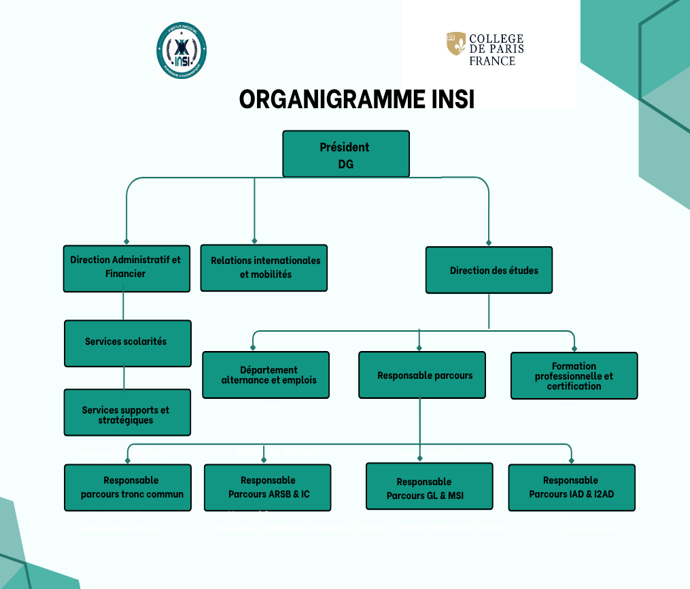
\includegraphics[width=10cm]{organigramme.png}
    \caption{Organigramme de l’INSI }
        \caption*{\textit{Source : INSI, 2025}} % n'apparaît pas dans la liste des figures
    \label{fig:organigramme}
\end{figure}

L'organigramme de l’INSI, en partenariat avec le Collège de Paris, est structuré autour d’une direction générale incarnée par le Président Directeur Général. Ce dernier assure la coordination de trois pôles principaux : la \textbf{Direction Administrative et Financière}, la \textbf{Direction des Études}, et le \textbf{Service des Relations Internationales et Mobilités}.

Le \textbf{Président Directeur Général} assure la direction stratégique de l’institut. Il supervise l’ensemble des activités pédagogiques, administratives et de développement. Il veille à la qualité de l’enseignement, à la bonne gestion des ressources humaines et matérielles, et représente l’établissement auprès des partenaires et autorités.

La \textbf{Direction Administrative et Financière} est chargée de la gestion des affaires internes, notamment à travers deux services essentiels : 
\begin{itemize}
    \item le \textbf{Service des scolarités}, qui s’occupe des dossiers étudiants, inscriptions et suivi académique,
    \item les \textbf{Services supports et stratégiques}, qui assurent un appui logistique, administratif et technologique à l’ensemble de l’institut.
\end{itemize}

Le \textbf{pôle des Relations Internationales et Mobilités} gère les échanges académiques avec l’étranger ainsi que les projets de mobilité étudiante ou enseignante. 

La \textbf{Direction des Études} supervise quant à elle l’ensemble des programmes pédagogiques et le corps enseignant. Elle travaille en étroite collaboration avec un \textbf{Responsable Parcours}, qui coordonne les différentes spécialisations proposées. Cette direction intègre également une \textbf{cellule Formation professionnelle et certification}, en charge des dispositifs de validation des compétences, des certifications professionnelles et des parcours de formation continue. Elle comprend aussi le \textbf{Département alternance et emplois}, responsable du suivi des étudiants en contrat d’alternance, des stages professionnels, et de l’insertion professionnelle.

Sous la responsabilité du \textbf{Responsable Parcours}, plusieurs responsables pédagogiques gèrent les différentes filières de formation :
\begin{itemize}
    \item le \textbf{parcours tronc commun}, qui regroupe les matières fondamentales partagées par tous les étudiants en début de cycle,
    \item le \textbf{parcours ARSB \& IC},
    \item le \textbf{parcours GL \& MSI},
    \item le \textbf{parcours IAD \& I2AD}.
\end{itemize}

D’autres structures, bien que non représentées sur cet organigramme, contribuent également de manière significative à la mission de l’INSI :
\begin{itemize}
    \item Le \textbf{Conseil de l’École}, regroupant des membres de l’équipe pédagogique et administrative. Il joue un rôle consultatif ou décisionnel sur les questions académiques : validation des programmes, suivi des résultats, discipline, méthodologie, etc.
    \item Le \textbf{Responsable de la formation en ligne}, qui conçoit et supervise les dispositifs d’apprentissage à distance. Il s’assure que les contenus en ligne sont accessibles, interactifs et conformes aux standards pédagogiques, tout en accompagnant enseignants et étudiants dans leur utilisation.
    \item L’\textbf{Association et les clubs étudiants}, qui encadrent et soutiennent les initiatives étudiantes, les clubs thématiques (informatique, innovation, sport, culture, etc.), et les événements organisés dans le cadre de la vie étudiante. Cela favorise l’engagement, le développement personnel et les compétences transversales des étudiants.
\end{itemize}

Cette structure témoigne d’une organisation à la fois pédagogique, administrative et tournée vers l’international et l’employabilité, assurant une formation complète et professionnalisante aux étudiants.
\section{Domaine de spécialisation}

INSI University propose des parcours académiques professionnalisants dans le domaine de l’informatique et des technologies numériques, articulés autour de licences professionnelles, de masters spécialisés, de formations professionnelles continues et d’opportunités de mobilité internationale.

\subsection{Licences professionnelles}

Les programmes de licence offrent une formation de base solide, axée sur la pratique, et préparant à une insertion rapide dans le monde professionnel :

\begin{itemize}
    \item \textbf{GL (Génie Logiciel)} : Conception, développement et maintenance d'applications logicielles.
    \item \textbf{ARSB (Administration Réseaux et Systèmes et Base de données)} : Gestion d’infrastructures informatiques, réseaux, serveurs et systèmes.
    \item \textbf{IAD (Intelligence Artificielle et Data Science)} : Introduction aux algorithmes d’IA, au traitement de données et à l’apprentissage automatique.
\end{itemize}

\subsection{Masters professionnels}

Les masters permettent d’approfondir les compétences techniques et managériales, en lien étroit avec les évolutions du secteur :

\begin{itemize}
    \item \textbf{MSI (Management des Systèmes d’Information)} : Pilotage de projets numériques, gouvernance des SI.
    \item \textbf{IC (Infrastructures et Cybersécurités)} : Sécurisation des systèmes, audit, réseaux avancés.
    \item \textbf{I2AD (Intelligence Artificielle, Analyse de Données et Automatisation)} : Applications avancées de l’IA, automatisation des processus et science des données.
\end{itemize}

\subsection{Formations professionnelles continues}

INSI University propose également des formations professionnelles continues, spécifiquement conçues pour les professionnels déjà en poste souhaitant approfondir leurs compétences ou se spécialiser dans l’un des domaines proposés.

Ces formations sont adaptées aux contraintes des professionnels (horaires flexibles, modules pratiques) et visent à renforcer leur employabilité ou à accompagner leur évolution de carrière.

\subsection{Mobilité internationale et double diplôme}

Dans une optique d’ouverture et de reconnaissance internationale, INSI propose à ses étudiants des opportunités de mobilité académique et de double diplôme, à partir de la deuxième année (L2) :

\begin{itemize}
    \item \textbf{Format hybride} : 6 mois de formation à Madagascar + 6 mois à l’étranger selon le parcours choisi.
    \item \textbf{Double diplôme en L3 ou M2} : En partenariat avec des institutions internationales telles que :
    \begin{itemize}
        \item Collège de Paris (France)
        \item Keyce Informatique (France)
        \item Eskills (Québec, Canada)
    \end{itemize}
\end{itemize}

\subsubsection*{Conditions d’éligibilité}
\begin{itemize}
    \item Niveau DALF C1 en français pour la mobilité vers des pays francophones.
    \item Niveau B2 ou C1 en anglais pour les destinations anglophones.
\end{itemize}

\section{Architectures des formations pédagogiques}

Le recrutement des étudiants à l’INSI s’effectue exclusivement par sélection de dossiers pour l’entrée en première année de Licence (L1), et par voie de concours pour l’admission en Master 1.

Au sein de l’INSI, une seule mention est proposée : \textbf{Informatique}, déclinée en trois parcours distincts aux niveaux Licence et Master.


\begin{table}[H]
\centering
\begin{tabular}{|l|l|}
\hline
\textbf{Licence} & \textbf{Master} \\
\hline
Génie Logiciel (GL) & Management des Systèmes d’Information (MSI) \\
\hline
Administration Réseaux, Systèmes et Bases de \\données (ARSB) & Infrastructures et Cybersécurités (IC) \\
\hline
Intelligence Artificielle et Data Science (IAD) & Intelligence Artificielle, Analyse de Données et \\Automatisation (I2AD) \\
\hline
\end{tabular}
\caption{Parcours Licence et Master proposés à l’INSI}
\caption*{\textit{Source : INSI, 2025}}
\label{tab:parcours}
\end{table} 

L’architecture des études à trois niveaux conformément au système LMD (Licence Master et Doctorat) permet les comparaisons et les équivalences académiques des diplômes au niveau international.\\
L = Licence (Bac + 3) = L1, L2, L3 = 6 semestres S1 à S6\\
M = Master (Bac + 5) = M1, M2 = 4 semestres S7 à S10\\
Le diplôme de licence est obtenu en 3 années des études après Baccalauréat. Et le diplôme de Master est obtenu en 2 ans après obtenu du diplôme de LICENCE.\\
Le MASTER PROFESSIONNEL est un diplôme destiné à la recherche emploi au terme des études.\\

\textbf{Spécificités pédagogiques} 
\begin{itemize}
    \item École d'alternance dès la L2 S4\\
    Alternance cours/entreprise pour une meilleure insertion
    \item Écoles connectées \& e-learning\\
    Plateforme numérique de formation, cloud intégré, Google Workspace\\
    Cours accessibles en ligne selon les parcours
    \item Pédagogie active \& par projets\\
    Hackathons, soutenances exposées, projets réels en entreprise
\end{itemize}

\textbf{VI. Relations de l’INSI avec les entreprises et les organismes} 
L’Institut National Supérieur en Informatique (INSI) entretient des liens étroits avec le monde professionnel. L’INSI collabore activement avec de nombreux organismes publics, semi-publics et privés, tant au niveau national qu’international. Cette collaboration se traduit concrètement par l’organisation régulière de stages obligatoires pour les étudiants, favorisant leur immersion professionnelle et leur employabilité.\\

Parmi les entreprises et institutions partenaires accueillant nos étudiants en stage chaque année :
\begin{itemize}
    \item Data Pulse Center
    \item RELIA Consulting
    \item Code Talent
    \item Bocasay
    \item Minimad
    \item Smartone AI
    \item NOVITY
    \item Eclosia Madagascar
    \item VISEO Groupe
    \item Océane Trade
    \item ACCES Banque
\end{itemize}

En plus des stages, l’INSI organise régulièrement des visites pédagogiques, des rencontres métiers et des projets collaboratifs avec plusieurs entreprises du secteur technologique et numérique. Ces activités permettent aux étudiants de mieux comprendre les réalités du terrain, d’échanger avec des professionnels et de s’ouvrir à l’environnement entrepreneurial.\\

Parmi les entreprises ayant accueilli ces initiatives :
\begin{itemize}
    \item NOVITY
    \item YAS Madagascar
    \item Smartone AI
    \item Eclosia Madagascar
    \item et d'autres acteurs majeurs du numérique à Madagascar
\end{itemize}

Cette dynamique de partenariat permanent constitue un pilier de la pédagogie à l’INSI, en lien avec son objectif de former des professionnels compétents, opérationnels et ancrés dans les besoins du marché.\\

\textbf{VII. Partenariat au niveau international} 
L’INSI s’est inscrit dans une dynamique d’ouverture à l’international grâce à son partenaire fondateur, ILO Madagascar, représentant de l’Organisation Internationale du Travail. Cette orientation se renforce aujourd’hui à travers des partenariats stratégiques avec des institutions académiques et des entreprises internationales, permettant à l’Institut de proposer une formation alignée sur les standards mondiaux.\\

L’INSI bénéficie actuellement de programmes de co-diplomation et de double diplôme en collaboration avec plusieurs établissements internationaux de renom :
\begin{itemize}
    \item Collège de Paris International
    \item Keyce Informatique (France)
    \item Eskills Academy (Québec, Canada)
    \item École Supérieure Polytechnique d’Antsiranana (ESPA) – pour une synergie régionale renforcée
\end{itemize}

Par ailleurs, à travers les stages annuels et projets pédagogiques, l’INSI collabore également avec des entreprises à dimension régionale ou mondiale :
\begin{itemize}
    \item VISEO Groupe
    \item Eclosia Madagascar (Groupe mauricien)
    \item Smartone AI
    \item NOVITY
\end{itemize}

\textbf{VIII. Parcours professionnels des diplômés} 
Les diplômés de la Licence en Informatique de l’INSI disposent d’un socle solide de compétences en programmation, systèmes, réseaux, bases de données et développement logiciel. Cette polyvalence leur permet d’intégrer directement le marché du travail ou de poursuivre en Master. À ce niveau, ils peuvent exercer en tant que :
\begin{itemize}
    \item Technicien système et réseau
    \item Développeur web / mobile (front-end ou back-end)
    \item Administrateur systèmes junior
    \item Technicien support IT
    \item Intégrateur / testeur logiciel
    \item Assistant en sécurité informatique
    \item Assistant en projets d’IA ou de data (selon profil)
\end{itemize}

Les stages annuels en entreprise leur offrent une première expérience professionnelle valorisante dans des structures variées : entreprises technologiques, banques, administrations, startups, ONG, etc.\\

La formation de Master proposée à l’INSI, grâce à ses parcours spécialisés, forme des professionnels capables d’intervenir sur des projets complexes, innovants et à dimension stratégique. Les débouchés varient selon la spécialisation choisie :

\textbf{Parcours Ingénierie logicielle, réseaux et systèmes :}
\begin{itemize}
    \item Ingénieur en développement logiciel / full-stack
    \item Architecte logiciel
    \item Ingénieur systèmes et réseaux
    \item Administrateur cloud / DevOps
    \item Chef de projet informatique
\end{itemize}

\textbf{Parcours Cybersécurité :}
\begin{itemize}
    \item Expert en sécurité des systèmes d'information
    \item Analyste SOC / CERT
    \item Auditeur en cybersécurité
    \item Responsable de la sécurité IT (RSSI)
\end{itemize}

\textbf{Parcours Intelligence Artificielle et Data :}
\begin{itemize}
    \item Data Scientist
    \item Data Analyst
    \item Ingénieur en Intelligence Artificielle
    \item Machine Learning Engineer
    \item Développeur d'applications intelligentes
    \item Consultant en IA
    \item Spécialiste en traitement automatique du langage naturel (TALN)
    \item Spécialiste en vision par ordinateur (Computer Vision)
\end{itemize}

Grâce aux partenariats internationaux et aux projets en entreprise, les diplômés du Master peuvent également prétendre à des postes dans des structures multinationales, ou poursuivre une carrière académique et de recherche (doctorat, enseignement supérieur).\\

\textbf{IX. Ressources humaines} 
L’INSI s’appuie sur une équipe pédagogique et administrative compétente, dynamique et engagée dans la réussite de ses étudiants. Ses ressources humaines se répartissent comme suit :
\begin{itemize}
    \item Président Directeur de l’INSI : Dr RAMASONDRANO Andriamanjaka
    \item Responsable parcours ARSB \& IC : Mr RATIANARISON Hery Mampionona
    \item Responsable parcours tronc commun : Dr RAKOTONDRAMANANA R, Sitraka
    \item Responsable parcours GL \& MSI : Mr ANDRIaAMIADANA TANTELY ANTOINE
    \item Responsable parcours IAD \& I2AD : par intérim PDG
    \item Nombres d'enseignants : 40
    \item Nombres des personnels administratives : 04
    \item Personnels d’appui : 6
\end{itemize}

\end{document}

